\documentclass{article}
\usepackage[utf8]{inputenc}
\usepackage[T1]{fontenc}
\usepackage[english]{babel}
\usepackage{amsmath}
\usepackage{amsthm}
\usepackage{tikz}
\usepackage{enumitem}\usepackage{systeme}
\begin{document}


\begin{center}
\section*{Esercizi d’esame Analisi Matematica 1}
Corso di Laurea in Scienze e Tecnologie informatiche\\
Dennis Antonio Amiranda
\end{center}

\section*{Abstract  }
Questo progetto vuole essere una trascrizione e revisione di alcuni esercizi che sono attinenti al corso di Analisi Matematica 1, con il fine di arricchire e raffinare la comprensione degli argomenti trattati. Gli esercizi svolti sono tre, due concernono la dimostrazione di due disuguaglianze, la prima e la seconda sono un caso specifico della inequality of arithmetic and geometric means (AM-GM inequality). Il terzo esercizio riguarda una funzione fratta, e uno studio estensivo delle sue proprietà.

%ESERCIZIO 6
\section*{Esercizio 6}
Dimostrare la seguente disuguaglianza
\[
\sqrt{ab} < \frac{a+b}{2} \quad \text{(6)}
\]
\begin{proof}
    Possiamo riscrivere la (6) nel seguente modo:
    \[
    a + b - 2\sqrt{a}\sqrt{b} > 0
    \]
    \[
    (\sqrt{a} - \sqrt{b})^2 > 0
    \]
    che è sempre positivo perché è un quadrato.
\end{proof}

%ESERCIZIO 7 
\section*{Esercizio 7}
Dimostrare che vale la seguente disuguaglianza
\[
\sqrt{n!} < \frac{n+1}{2} \quad (n! = 1 \cdot 2 \cdot 3 \cdots n)
\]
\begin{proof}
    Dalla definizione di \(n!\), possiamo riscriverlo come
    \[
    n! = \sqrt{1} \cdot \sqrt{1} \times \sqrt{2} \cdot \sqrt{2} \times \ldots \times \sqrt{n} \cdot \sqrt{n}
    \]
    \[
    = \prod_{k=1}^{n} k = \prod_{k=1}^{n} \sqrt{k} \cdot \sqrt{k}
    \]
    \[
    = (\sqrt{1} \cdot \sqrt{n}) \cdot (\sqrt{2} \cdot \sqrt{n-1}) \cdot \ldots \cdot (\sqrt{n-1} \cdot \sqrt{2}) \cdot (\sqrt{n} \cdot \sqrt{1})
    \]
    \[
    = \prod_{k=1}^{n} \sqrt{k} \cdot \sqrt{n-k+1}
    \]
    \[
    = \sqrt{1 \cdot n} \times \sqrt{2(n-1)} \times \ldots \times \sqrt{2(n-1)} \times \sqrt{1 \cdot n} 
    \]
    Possiamo utilizzare adesso la disuguaglianza (6), infatti per ogni radice singola dell’equazione scritta poc’anzi, vale la seguente disuguaglianza
    \[
    n! = x < \frac{1+n}{2} \cdot \ldots \cdot \frac{1+n}{2} = \left(\frac{1+n}{2}\right)^n
    \]
    Adesso, poiché vale la diseguaglianza tra \(x\) e l’espressione posta sopra, possiamo prendere la radice \(n\)-esima di entrambi i membri, ottenendo:
    \[
    \sqrt{n!} < \frac{n+1}{2}
    \]
\end{proof}

%ESERCIZIO 15
\section*{Esercizio 15}
In un piano, riferito a un sistema di assi cartesiani ortogonali (\(Oxy\)), è assegnata la seguente famiglia di funzioni:
\[
f(x) = \frac{ax^2 + b|x| + c}{d - x} \quad \text{con } a, b, c, d \in R
\]

\begin{enumerate}[label=\Roman*] 
    \item Determinare in modo tale che la curva che rappresenta la funzione abbia
        \begin{itemize}
            \item Asintoto verticale $x = 2$;
            \item Asintoto obliquo con coefficiente angolare $m = -1$;
            \item Passi per $A(3, 0)$, $B(-6, 0)$.
        \end{itemize}
    
    \item Studiare la funzione richiesta in I) nel suo campo di esistenza e tracciare il grafico \(\gamma\), dopo aver classificato eventuali punti di non derivabilità.
    
    \item Dopo aver dimostrato che il punto \(A\) d’intersezione di \(\gamma\) con l’asse delle ordinate è un punto angoloso, scrivere le equazioni delle tangenti in \(A\).
    
    \item Calcolare l’area del dominio piano delimitato da \(\gamma\), l’asse delle ascisse e le rette \(x = -2\) e \(x = -1\).
    
    \item Dimostrare che la funzione \(f(x) = \frac{x^2 + 9|x| + 18}{2 - x}\) verifica le ipotesi del teorema di Lagrange nell’intervallo \([0, 1]\) e determinare i “punti di Lagrange”. Perché non verifica Lagrange nell’intervallo \([-3, 1]\)?
\end{enumerate}
\textit{Svolgimento}\\
PARTE I.
Per avere un asintoto in \(x = 2\), dobbiamo avere che \(2\) sia nel dominio, cioè
\[
d - 2 = 0 \quad \Rightarrow \quad d = 2.
\]
Per l’obliquo invece,
\[
\lim_{x \to \infty} \frac{ax^2 + b|x| + c}{d - x} \cdot \frac{1}{x} = \lim_{x \to \infty} \frac{ax^2}{-x} \cdot \frac{1}{x} = -a.
\]
Allora deve essere che \(a = 1\).
Poiché \(A(3, 0) \in \gamma\) e \(B(-6, 0) \in \gamma\), otteniamo:
\[
\systeme*{A(3;0) \in \gamma, B(-6;0)\in \gamma}  \Rightarrow \quad
\systeme*{\frac{9+3b+c}{2-3} = 0, \frac{36+6b+c}{2+6} = 0} \Rightarrow \quad
\systeme*{-3b -9 = c, 36 + 3b -9  = 0} 
\] 
\[
\systeme*{b = -9, c = 18} 
\]
\\
PARTE II.
studiamo
$f(x) = \frac{x^2 - 9|x| + 18}{2-x}$, il suo campo di esistenza è $R-\{2\}$. La funzione ha un valore assoluto, dobbiamo allora studiarne l'andamento in due casi: per $x \in ]-\infty, 0[$ e $x \in [0, \infty[ - \{2\}$.
Nel caso 1 abbiamo che $f(x) = \frac{x^2 + 9x + 18}{2-x}$, studiamo il segno, $x^2 + 9x + 18 \geq 0$ e $2-x > 0$
che ci danno, come soluzioni, $x \leq -6 \land x \geq -3$ e $x < 2$, studiando il grafico, otteniamo
\\\\
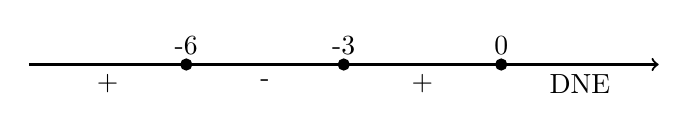
\begin{tikzpicture}
\draw[thick, ->] (0,0) -- (8,0);
\filldraw (2,0) circle (2pt) node[anchor=south]{-6};
\filldraw (1,0) node[anchor=north]{+};
\filldraw (4,0) circle (2pt) node[anchor=south]{-3};
\filldraw (3,0) node[anchor=north]{-};
\filldraw (6,0) circle (2pt) node[anchor=south]{0};
\filldraw (5,0) node[anchor=north]{+};
\filldraw (7,0) node[anchor=north]{DNE};
\end{tikzpicture}
\\\\
quindi abbiamo che $x \in ]-\infty, -6]$ e $x \in [-3, 0[$
abbiamo che interseca l'asse y in 9, perché $f(0) = 9$.
Inoltre, non ha asintoti orizzontali, poiché
\[
\lim_{x \to -\infty} f(x) = +\infty
\]
per l'asintoto obliquo abbiamo m = -1 per ipotesi, ci basta calcolare in questo caso 
\[
\lim_{x\to-\infty} f(x)-x = \lim_{x\to-\infty}\frac{x^2 + 9x + 18}{2-x} - \frac{2x-4}{2-x}
\]
\[
\lim_{x\to-\infty}\frac{11x+18}{2-x} = -11
\]

quindi $y = -x - 11$ è l'asintoto obliquo per $-\infty$.

derivata prima, per la regola di derivazione di una frazione abbiamo che:
\[
f'(x) = \frac{(2x+9)(2-x)+x^2+9x+18}{(2-x)^2} = \frac{-x^2+4x+36}{(2-x)^2}
\]
per il segno,
\[
x^2-4x-36 \leq 0
\]
\[
(2-x)^2 > 0
\]
che hanno soluzione $x \geq 2-2\sqrt{10} \land x \leq 2+2\sqrt{10}$ e $\forall x \in R-\{2\}$, quindi
\\\\
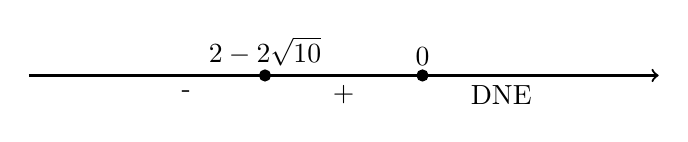
\begin{tikzpicture}
\draw[thick, ->] (0,0) -- (8,0);
\filldraw (3,0) circle (2pt) node[anchor=south]{$2-2\sqrt{10}$};
\filldraw (2,0) node[anchor=north]{-};
\filldraw (4,0) node[anchor=north]{+};
\filldraw (5,0) circle (2pt) node[anchor=south]{0};
\filldraw (6,0) node[anchor=north]{DNE};
\end{tikzpicture}
\\\\

per la derivata seconda, per la regola di derivazione di una frazione abbiamo che:
\[
f''(x) = \frac{(-2x+4)(2-x)^2+2(2-x)(-x^2+4x+36)}{(2-x)^4} 
\]
\[
= \frac{2(2-x)(x^2-4x+4-x^2+4x+36)}{(2-x)^4}
= \frac{80}{(2-x)^3}
\]
la quale si vede chiaramente in base al dominio non positivo, essere positiva per ogni x: la funzione è sempre convessa.\\
studiamo ora $f(x) = \frac{x^2 - 9x + 18}{2-x}$ in $x \in [0, \infty[ - \{2\}$.
per il segno,
\[
x^2-9x+18 \geq 0
\]
\[
x < 2
\]
abbiamo che $f(0) = 9$, allora abbiamo che la funzione è continua in 0. Per il segno 
$x \leq 3 \land x \geq 6 $ e $x < 2$, quindi
\\\\
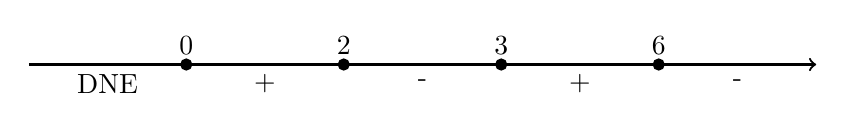
\begin{tikzpicture}
\draw[thick, ->] (0,0) -- (10,0);
\filldraw (2,0) circle (2pt) node[anchor=south]{0};
\filldraw (1,0) node[anchor=north]{DNE};
\filldraw (4,0) circle (2pt) node[anchor=south]{2};
\filldraw (3,0) node[anchor=north]{+};
\filldraw (6,0) circle (2pt) node[anchor=south]{3};
\filldraw (5,0) node[anchor=north]{-};
\filldraw (7,0) node[anchor=north]{+};
\filldraw (8,0) circle (2pt) node[anchor=south]{6};
\filldraw (9,0) node[anchor=north]{-};
\end{tikzpicture}
\\\\
Non possiede asintoti orizzontali,
\[
\lim_{x \to +\infty} f(x) = -\infty
\]
Invece ha asintoti obliqui.
\[
\lim_{x \to +\infty} f(x) \cdot \frac{1}{x} = -1
\]
\[
\lim_{x \to +\infty} f(x) -x =  7
\]
allora $y = -x + 7$ è asintoto obliquo. La derivata prima è\\
\[f'(x) = \frac{(2x-9)(2-x) + x^2 -9x + 18}{(2-x)^2} = \frac{-x^2 + 4x}{(2-x)^2}
\]
Studiamone il segno:
\[
x^2 - 4x \leq 0
\]
\[
(2-x)^2 > 0
\]
\\
le due equazioni danno soluzioni: $0 \leq x  \leq 4 \land \forall x \in R-\{2\}$ quindi, usando la tabella dei segni
\\\\
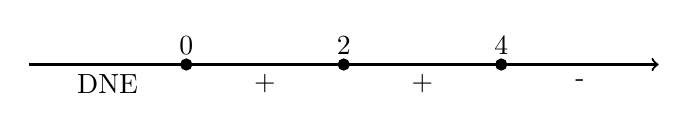
\begin{tikzpicture}
\draw[thick, ->] (0,0) -- (8,0);
\filldraw (2,0) circle (2pt) node[anchor=south]{0};
\filldraw (1,0) node[anchor=north]{DNE};
\filldraw (4,0) circle (2pt) node[anchor=south]{2};
\filldraw (3,0) node[anchor=north]{+};
\filldraw (6,0) circle (2pt) node[anchor=south]{4};
\filldraw (5,0) node[anchor=north]{+};
\filldraw (7,0) node[anchor=north]{-};
\end{tikzpicture}
\\\\
Abbiamo che $f(4) = 1$, che è un punto di massimo. Inoltre  il punto $0$ è angoloso, infatti
\[
\lim_{x \to 0^-} f'(x) =  9 \ne \lim_{x \to 0^+} f'(x) =  0
\]
Infatti $f$ è definita come $f'(x) = \frac{-x^2+4x+36}{(2-x)^2}$ da sinistra, e $f'(x) =  \frac{-x^2 + 4x}{(2-x)^2}$ da destra. Per la derivata seconda:
\[
f''(x) = \frac{('2x+4)(2-x)^2 + 2(2-x)(-x^2+4x)}{(2-x)^2} = \frac{2(2-x)(4)}{(2-x)^4}
\]
\[
= \frac{8}{(2-x)^3}
\]
cui banalmente vale,
\\\\
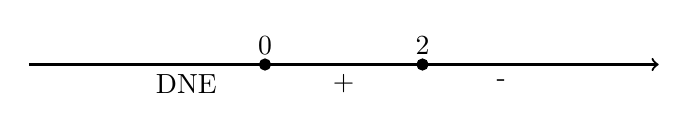
\begin{tikzpicture}
\draw[thick, ->] (0,0) -- (8,0);
\filldraw (3,0) circle (2pt) node[anchor=south]{0};
\filldraw (2,0) node[anchor=north]{DNE};
\filldraw (4,0) node[anchor=north]{+};
\filldraw (5,0) circle (2pt) node[anchor=south]{2};
\filldraw (6,0) node[anchor=north]{-};
\end{tikzpicture}
\\\\
PARTE III.
Come dimostrato nel punto II. 0 appartiene a $f$, abbiamo $A(0,9)$ e quindi interseca l'asse delle ordinate in 9. La retta tangente in $A$ sarà: $y = f'(x)(x-x_0) +f(x_0) \implies y = 9(x-0) + 9 \implies y = 9x+ 9$.
\\\\PARTE IV. dobbiamo calcolare l'integrale 
\[
A(D) = \int_{-2}^1 \frac{x^2 - 9|x| + 18}{2-x}dx =  \int_{-2}^0\frac{x^2 + 9x + 18}{2-x}dx + 
 \int_{0}^1\frac{x^2 - 9x + 18}{2-x}dx
\]
per il primo, possiamo dividere per ruffini, e otteniamo
\\\\
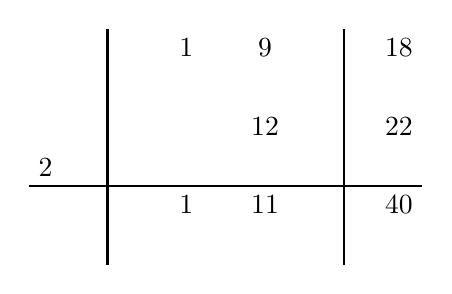
\begin{tikzpicture}
\draw[thick] (0,0) -- (5,0);
\draw[thick] (1,-1) -- (1, 2);
\draw[thick] (4,-1) -- (4 , 2);
\filldraw (2,0) node[anchor=north]{1};
\filldraw (0,0) node[anchor=south west]{2};
\filldraw (3,0) node[anchor=north]{11};
\filldraw (2,2) node[anchor=north]{1};
\filldraw (3,2) node[anchor=north]{9};
\filldraw (3,1) node[anchor=north]{12};
\filldraw (5,2) node[anchor=north east]{18};
\filldraw (5,1) node[anchor=north east]{22};
\filldraw (5,0) node[anchor=north east]{40};
\end{tikzpicture}
\\\\
\[
\int \frac{x^2 + 9x + 18}{2-x}dx = -\int \frac{(2-x)(x+11)}{(2-x)}dx  -40\int\ \frac{1}{x-2}dx
\]
\[
= -\int (x+11) dx - 40ln|x-2| = -\frac{(x+11)^2}{2} - 40ln|x-2|
\]
Parimente per il secondo abbiamo
\\\\
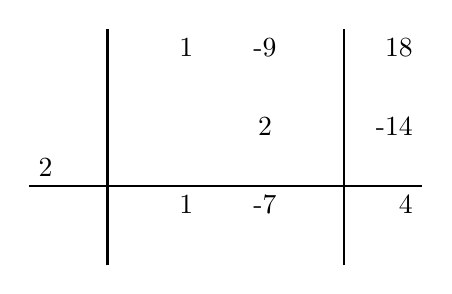
\begin{tikzpicture}
\draw[thick] (0,0) -- (5,0);
\draw[thick] (1,-1) -- (1, 2);
\draw[thick] (4,-1) -- (4 , 2);
\filldraw (2,0) node[anchor=north]{1};
\filldraw (0,0) node[anchor=south west]{2};
\filldraw (3,0) node[anchor=north]{-7};
\filldraw (2,2) node[anchor=north]{1};
\filldraw (3,2) node[anchor=north]{-9};
\filldraw (3,1) node[anchor=north]{2};
\filldraw (5,2) node[anchor=north east]{18};
\filldraw (5,1) node[anchor=north east]{-14};
\filldraw (5,0) node[anchor=north east]{4};
\end{tikzpicture}
\\\\
\[
\int \frac{x^2 - 9x + 18}{2-x}dx = -\int \frac{(2-x)(x-7)}{(2-x)}dx  -4\int\ \frac{1}{x-2}dx
\]
\[
= -\int (x-7) dx - 4ln|x-2| = -\frac{(x-7)^2}{2} - 4ln|x-2|
\]
per la formula fondamentale del calcolo integrale dobbiamo sicché calcolare
\[
\left[ -\frac{(x+11)^2}{2} - 40ln|x-2|\right]_{-2}^0 + \left[ -\frac{(x-7)^2}{2} - 4ln|x-2|\right]_{0}^1 = 
\]
\[
-\frac{121}{2} - 40ln(2) + \frac{81}{2} + 40ln(4) -18 + \frac{49}{2} + 4ln(2) =
\]
\[
\frac{9}{2} - 18 - 35ln(2) + 80ln(2) \implies A(D) = 44ln(2) -\frac{27}{2}
\]
\\\\
PARTE V. abbiamo dimostrato che è $f(x)$ è continua in tutto $R-\{2\}$,  per il teorema di lagrange $\exists c \in ]0,1[$ tale che
\[
\frac{-c^2+4c}{(2-c)^2} = \frac{f(1)-f(0)}{1-0} \implies
\]
\[
-c^2 + 4c = 4 -4c + c^2, 
\]
\[
2c^2 -8c + 4 = 0 \implies c^2 - 4c + 2 = 0
\]
dalla quale otteniamo,
$c = 2\pm2\sqrt{2}$ nell'intervallo $]0,1[$ ci da $c = 2-\sqrt{2}$
la funzinoe non è derivabile in $[-3;1]$, non sono verificate le ipotesi del teorema di Lagrange, infatti $f(x)$ non è derivabile in $0 \in ]-3,1[$.
\begin{figure}
    \centering
    \includegraphics[width=0.6\linewidth]{image2.png}
    \caption{grafico della funzione}
    \label{fig:enter-label}
\end{figure}
\begin{figure}
    \centering
    \includegraphics[width=0.6\linewidth]{image3.png}
    \caption{asintoti}
    \label{fig:enter-label}
\end{figure}
\begin{figure}
    \centering
    \includegraphics[width=0.6\linewidth]{image.png}
    \caption{area dell'integrale}
    \label{fig:enter-label}
\end{figure}
\end{document}
